\documentclass[a4paper, 12pt]{article}%тип документа

%отступы
\usepackage[left=2cm,right=2cm,top=2cm,bottom=3cm,bindingoffset=0cm]{geometry}
\setlength{\parindent}{5ex}

%Русский язык
\usepackage[T2A]{fontenc} %кодировка
\usepackage[utf8]{inputenc} %кодировка исходного кода
\usepackage[english,russian]{babel} %локализация и переносы

%Вставка картинок
\usepackage{graphicx}
\graphicspath{{pictures/}}
\DeclareGraphicsExtensions{.pdf,.png,.jpg}

%Графики
\usepackage{pgfplots}
\pgfplotsset{compat=1.9}

%Математика
\usepackage{amsmath, amsfonts, amssymb, amsthm, mathtools}

%Таблицы
\usepackage{longtable} 
\usepackage{float}

%Римские цифры
\newcommand{\RomanNumeralCaps}[1]{\uppercase\expandafter{\romannumeral#1}}

\usepackage{multirow}


\begin{document}
	\begin{titlepage}
		\begin{center}
			\textsc{Федеральное государственное автономное образовательное учреждение высшего образования«Московский физико-технический институт (национальный исследовательский университет)»\\[5mm]
			}
			
			\vfill
			
			\textbf{Отчёт по лабораторной работы 3.6.1\\[3mm]
				Спектральный анализ электрических сигналов
				\\[50mm]
			}
			
		\end{center}
		
		\hfill
		\begin{minipage}{.5\textwidth}
			Выполнил студент:\\[2mm]
			Сериков Василий Романович\\[2mm]
			группа: Б03-102\\[5mm]
			
		\end{minipage}
		\vfill
		\begin{center}
			Москва, 2022 г.
		\end{center}
		
	\end{titlepage}
	
	\newpage
	\textbf{Аннотация}\\
	
	
	\textbf{Цель работы: }\\
	Изучить спектральный состав периодических электрических сигналов.\\
	
	
	\textbf{В работе используются: }\\
	Генератор сигналов произвольной формы, цифровой осциллограф с функцией быстрого преобразования Фурье.\\
	
	\textbf{Теоретические сведения: } \\
	
	\textit{Разложение сложных сигналов на периодические колебания}\\
	
	Используется разложение в сумму синусов и косинусов с различными аргументами или, как чаще его называют, \textit{разложение в ряд Фурье}.
	
	Пусть задана функция $f(t)$, которая периодически повторяется с частотой $\Omega_1 = \dfrac{2\pi}{T}$, где $T$ --- период повторения импульсов. Её разложение в ряд Фурье имеет вид 
	\begin{equation}
		f(t) = \dfrac{a_0}{2} + \sum\limits_{n = 1}^{\infty}\left[a_n \cos \left(n \Omega_1t\right) + b_n \sin \left(n \Omega_1t\right)\right]
	\end{equation}
	или
	\begin{equation}
		f(t) = \dfrac{a_0}{2} + \sum\limits_{n = 1}^{\infty}A_n \cos \left(n\Omega_1t-\psi_n\right).
	\end{equation}
	Если сигнал чётен относительно $t=0$, в тригонометрической записи остаются только члены с косинусами. Для нечетной наоборот.
	
	Коэффициенты определяются по формуле
	\begin{equation}
		\begin{array}{c}
			a_n  = \dfrac{2}{T}\int\limits_{t_1}^{t_1+T}f(t)\cos\left(n \Omega_1 t\right) dt,\\
			\\
			b_n = \dfrac{2}{T}\int\limits_{t_1}^{t_1+T}f(t)\sin\left(n \Omega_1 t\right) dt.
		\end{array}
	\end{equation}
	Здесь $t_1$ --- время, с которого мы начинаем отсчет.
	
	Сравнив формулы $(1)$ и $(2)$ можно получить выражения для $A_n$  и $\psi_n$:
	\begin{equation}
		\begin{array}{l}
			A_n = \sqrt{a_n^2+b_n^2},\\
			\psi_n = \arctan \dfrac{b_n}{a_n}.
		\end{array}
	\end{equation}
	\newpage
	\textit{Периодическая последовательность прямоугольных импульсов}\\
	
	\begin{figure}[H]
		\center{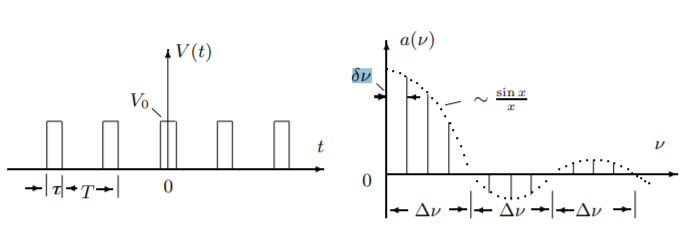
\includegraphics[scale=0.9]{2.png}}.
		\caption{Изображение прямоугольных импульсов и их спектров.}
	\end{figure}
	Введем величину: $\Omega_1 = \dfrac{2\pi}{T}$,
	где $T$ --- период повторения импульсов.
	
	Коэффициенты при косинусных составляющих будут равны
	\begin{equation}
		a_n = \dfrac{2}{T}\int\limits_{-\tau/2}^{\tau/2}V_0\cos\left(n\Omega_1 t\right)dt = 2V_0\dfrac{\tau}{T}\dfrac{\sin\left(n\Omega_1\tau/2\right)}{n\Omega_1\tau/2} \sim \dfrac{\sin x}{x}.
	\end{equation}
	
	Здесь $V_0$ - амплитуда сигнала.
	
	Поскольку наша функция четная, то $b_n = 0$. 
	
	Пусть $T$ кратно $\tau$. Тогда введем ширину спектра, равную $\Delta \omega$ --- расстояние от главного максимума до первого нуля огибающей, возникающего, как нетрудно убедиться при $n = \dfrac{2\pi}{\tau \Omega_1}$. При 
	этом
	\begin{equation}
		\Delta \omega \tau \simeq 2\pi \Rightarrow \Delta \nu \Delta t \simeq 1.
	\end{equation}\\

	\textit{Периодическая последовательность цугов}\\
	
	\begin{figure}[H]
		\center{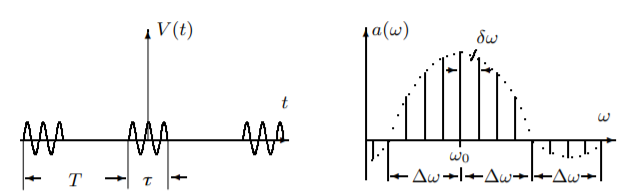
\includegraphics[scale=0.9]{3.png}}
		\caption{Изображение цугов и их спектра}
	\end{figure}
	Возьмём цуги колебания $V_0 \cos(\omega_0 t)$ с длительностью цуга $\tau$ и периодом повторений $T$.\\
	Функция $f(t)$ снова является четной относительно $t = 0$. Коэффициент при $n$-ой гармонике согласно формуле $(3)$ равен
	\begin{equation}
		a_n = \dfrac{2}{T}\int\limits_{-\tau/2}^{\tau/2}V_0 \cos \left(\omega_0t\right) \cdot \cos\left(n \Omega_1t\right)dt = V_0 \dfrac{\tau}{T}\left( \dfrac{\sin\left[\left(\omega_0 - n \Omega_1\right)\dfrac{\tau}{2}\right]}{\left( \omega_0 - n \Omega_1\right) \dfrac{\tau}{2}} + \dfrac{\sin\left[\left(\omega_0 + n \Omega_1\right)\dfrac{\tau}{2}\right]}{\left( \omega_0 + n \Omega_1\right) \dfrac{\tau}{2}}\right).
	\end{equation}
	Пусть $T$ кратно $\tau$. Тогда спектры последовательности прямоугильных сигналов и цугов аналогичны, но максимумы сдвинуты на $\omega_0$.\\
	
	\textit{Амплитудно-модулированные колебания}\\
	
	\begin{figure}[H]
		\center{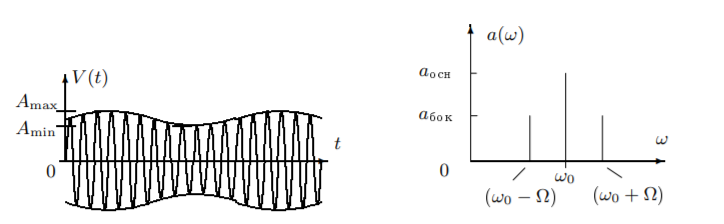
\includegraphics[scale=0.9]{4.png}}
		\caption{Изображение АМ колебаний и их спектра.}
	\end{figure}
	Рассмотрим гармонические колебания высокой частоты $\omega_0$, амплитуда которых медленно меняется по гармоническому закону с частотой $\Omega \ll \omega_0$.
	\begin{equation}
		f(t) = A_0 \left[1+m\cos \Omega t\right] \cos \omega_0 t.
	\end{equation}
	Коэффициент $m$ называется \textit{глубиной модуляции}. При $m < 1$ амплитуда меняется от минимальной $A_{min} = A_0(1-m)$ до максимальной $A_{max} = A_0(1+m)$. Глубина модуляции может быть представлена в виде
	\begin{equation}
		m = \dfrac{A_{max}-A_{min}}{A_{max}+A_{min}}.
	\end{equation}
	Простым тригонометрическим преобразованием уравнения $(8)$ можно найти спектр колебаний
	\begin{equation}
		f(t) = A_0 \cos \omega_0t + \dfrac{A_0m}{2} \cos \left(\omega_0 + \Omega\right)t + \dfrac{A_0m}{2}\cos\left(\omega_0 - \Omega\right)t.
	\end{equation}
	
	
	\newpage
	
	\textbf{Ход работы и обработка результатов.}\\
	
	\textbf{Исследование спектра периодической последовательности
		прямоугольных импульсов}
	\begin{enumerate}
	
	\item Проведем серию измерений ширины спектра $\Delta\nu$ от времени импульса $\tau$ при фиксированной частоте $\nu_{\text{повт}} = 1 $ кГц. Полученные данные занесем в таблицу и построим график зависимости $\Delta\nu(1/\tau)$
	

\begin{longtable} {|c|c|c|c|c|c|c|c|}
 	\hline
 	$\Delta\nu$, кГц& 49,9 & 25,0 & 16,6 & 12,5 & 9,9 & 8,5 & 7  \\ \hline
 	$\tau$, мкс & 20 & 40 & 60 & 80 & 100 & 120 & 140 \\ \hline
 	\caption{Зависимость ширины спектра от времени импульса.}
\end{longtable}


	
\begin{figure}[H]
	\center{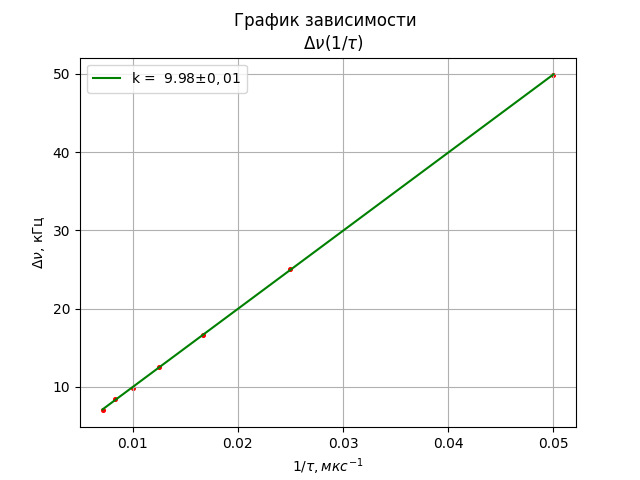
\includegraphics[scale=0.9]{v(t).png}}
	\caption{График зависимости $\Delta\nu(1/\tau)$.}
\end{figure}
	
	
\newpage

\begin{figure}[H]
	\center{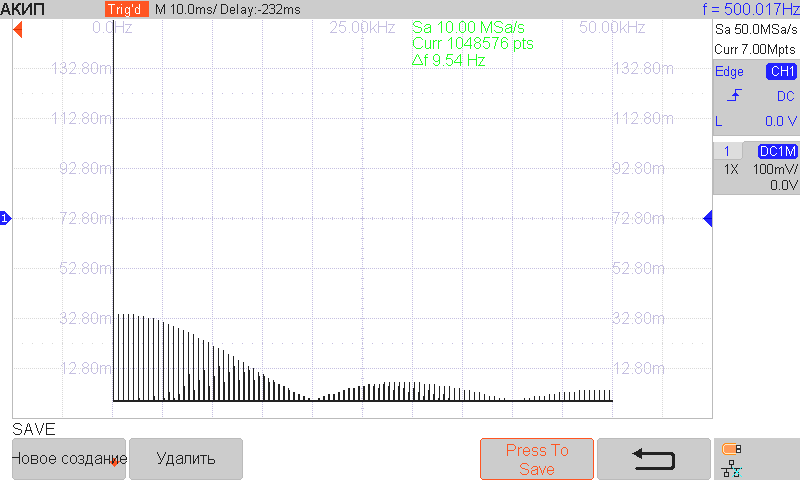
\includegraphics[scale=0.4]{0.5кгц50с.png}}
	\caption{$\nu_{\text{повт}} = 0,5$ кГц, $\tau$ = 50c}
\end{figure}
	
\begin{figure}[H]
	\center{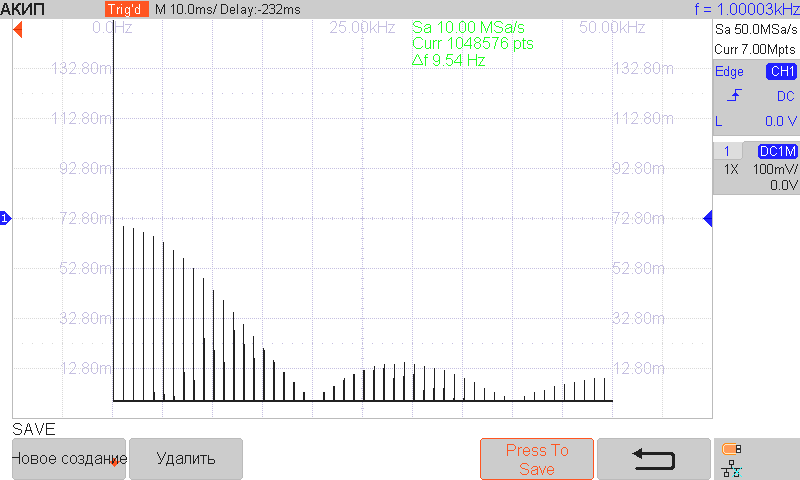
\includegraphics[scale=0.4]{1кгц50с.png}}
	\caption{$\nu_{\text{повт}} = 1$ кГц, $\tau$ = 50c}
\end{figure}

\begin{figure}[H]
	\center{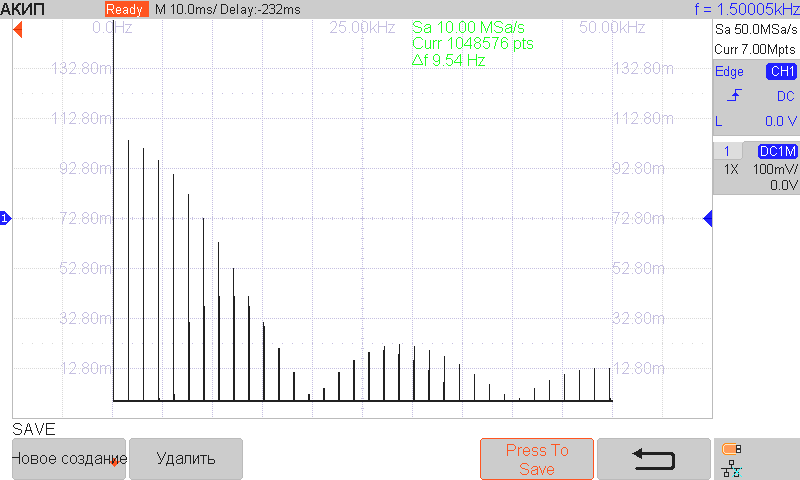
\includegraphics[scale=0.4]{1.5кгц50с.png}}
	\caption{$\nu_{\text{повт}} = 1,5$ кГц, $\tau$ = 50c}
\end{figure}

	\newpage

\begin{figure}[H]
	\center{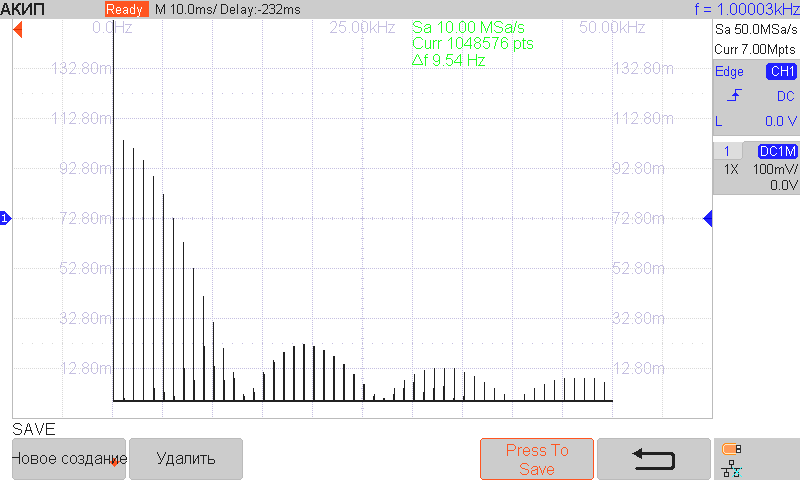
\includegraphics[scale=0.5]{1кгц75с.png}}
	\caption{$\nu_{\text{повт}} = 1$ кГц, $\tau$ = 75c}
\end{figure}
	
\begin{figure}[H]
	\center{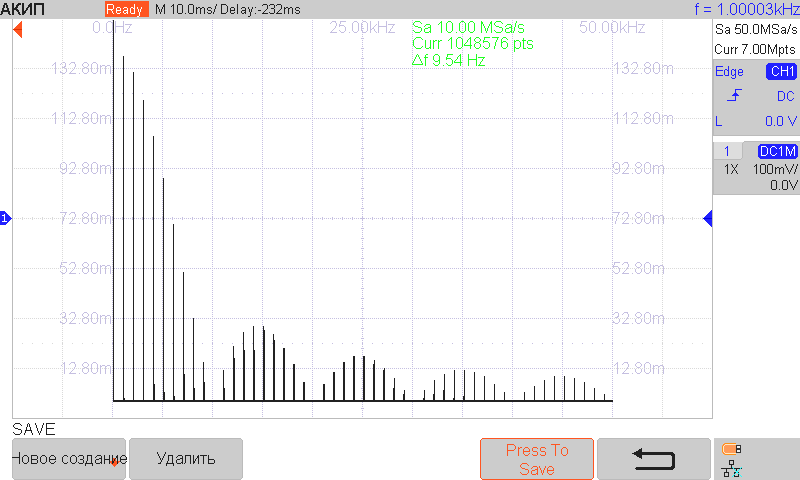
\includegraphics[scale=0.5]{1кгц100с.png}}
	\caption{$\nu_{\text{повт}} = 1$ кГц, $\tau$ = 100c}
\end{figure}

	
\newpage
	
\textbf{Исследование спектра периодической последовательности цугов}

\item При фиксированных параметрах $\nu$ = 50 кГц и N = 5 измерим зависимость расстояния $\delta\nu$ между соседними спектральными компонентами сигнала от периода T повторения импульсов. Полученные данные занесем в таблицу и построим график зависимости $\delta\nu(1/T)$
	
\begin{longtable} {|c|c|c|c|c|c|c|c|c|c|c|c|c|}
	\hline
	$\delta\nu$, кГц& 1,20 & 0,90 & 0,76 & 0,60 & 0,56 & 0,52 & 0,40 & 0,32 & 0,30 & 0,24 & 0,22 & 0,2 \\ \hline
	$T$, мс & 1 & 1,2 & 1,4 & 1,6 & 1,8 & 2,0 & 2,5 & 3,0 & 3,5 & 4,0 & 4,5 & 5,0 \\ \hline
	\caption{Зависимость расстояния между соседними
		спектральными компонентами сигнала от периода повторения импульсов.}
\end{longtable}
	
\begin{figure}[H]
	\center{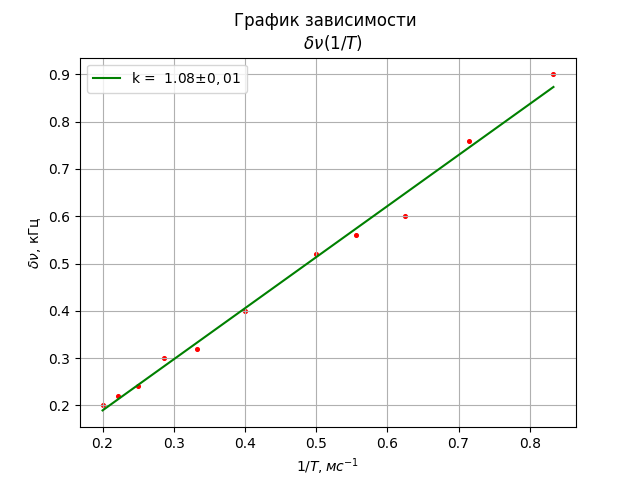
\includegraphics[scale=1]{v(T1).png}}
	\caption{График зависимости $\delta\nu(1/T)$}
\end{figure}
	
\end{enumerate}
	
	
	\textbf{Обсуждение результатов и выводы: }\\
	
	В данной работе мы изучили спектры периодической последовательности
	прямоугольных импульсов и периодической последовательности цугов. Для каждого спектра определили зависимость ширины $\delta \nu$ спектра от времени $\tau$, построили графики зависимость $\delta\nu(1/\tau)$ и подтвердили таким образом соотношение неопределенности $\delta\nu \cdot \tau = 1$
	
	
	
	
\end{document}